\documentclass[ignorenonframetext,]{beamer}
\setbeamertemplate{caption}[numbered]
\setbeamertemplate{caption label separator}{: }
\setbeamercolor{caption name}{fg=normal text.fg}
\beamertemplatenavigationsymbolsempty
\usepackage{lmodern}
\usepackage{amssymb,amsmath}
\usepackage{ifxetex,ifluatex}
\usepackage{fixltx2e} % provides \textsubscript
\ifnum 0\ifxetex 1\fi\ifluatex 1\fi=0 % if pdftex
  \usepackage[T1]{fontenc}
  \usepackage[utf8]{inputenc}
\else % if luatex or xelatex
  \ifxetex
    \usepackage{mathspec}
  \else
    \usepackage{fontspec}
  \fi
  \defaultfontfeatures{Ligatures=TeX,Scale=MatchLowercase}
\fi
% use upquote if available, for straight quotes in verbatim environments
\IfFileExists{upquote.sty}{\usepackage{upquote}}{}
% use microtype if available
\IfFileExists{microtype.sty}{%
\usepackage{microtype}
\UseMicrotypeSet[protrusion]{basicmath} % disable protrusion for tt fonts
}{}
\newif\ifbibliography
\hypersetup{
            pdftitle={Deep learning pour et par les nuls},
            pdfauthor={C. Ambroise et S. Donnet pour HappyR},
            pdfborder={0 0 0},
            breaklinks=true}
\urlstyle{same}  % don't use monospace font for urls
\usepackage{graphicx,grffile}
\makeatletter
\def\maxwidth{\ifdim\Gin@nat@width>\linewidth\linewidth\else\Gin@nat@width\fi}
\def\maxheight{\ifdim\Gin@nat@height>\textheight0.8\textheight\else\Gin@nat@height\fi}
\makeatother
% Scale images if necessary, so that they will not overflow the page
% margins by default, and it is still possible to overwrite the defaults
% using explicit options in \includegraphics[width, height, ...]{}
\setkeys{Gin}{width=\maxwidth,height=\maxheight,keepaspectratio}

% Prevent slide breaks in the middle of a paragraph:
\widowpenalties 1 10000
\raggedbottom

\AtBeginPart{
  \let\insertpartnumber\relax
  \let\partname\relax
  \frame{\partpage}
}
\AtBeginSection{
  \ifbibliography
  \else
    \let\insertsectionnumber\relax
    \let\sectionname\relax
    \frame{\sectionpage}
  \fi
}
\AtBeginSubsection{
  \let\insertsubsectionnumber\relax
  \let\subsectionname\relax
  \frame{\subsectionpage}
}

\setlength{\parindent}{0pt}
\setlength{\parskip}{6pt plus 2pt minus 1pt}
\setlength{\emergencystretch}{3em}  % prevent overfull lines
\providecommand{\tightlist}{%
  \setlength{\itemsep}{0pt}\setlength{\parskip}{0pt}}
\setcounter{secnumdepth}{0}

\title{Deep learning pour et par les nuls}
\author{C. Ambroise et S. Donnet pour HappyR}
\date{Rencontres R. Rennes. Juillet 2018}

\begin{document}
\frame{\titlepage}

\section{Introduction : apprentissage
supervisé}\label{introduction-apprentissage-supervise}

\begin{frame}{Exemple : reconnaissance de chiffres}

\begin{figure}
\centering
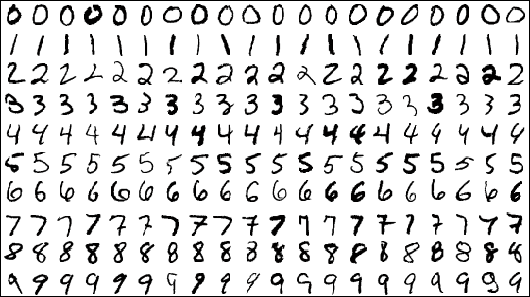
\includegraphics{mnist.png}
\caption{Reconnaissance de chiffres écrits à la main}
\end{figure}

\end{frame}

\begin{frame}{Exemple : reconnaissance de chiffres}

\begin{figure}
\centering
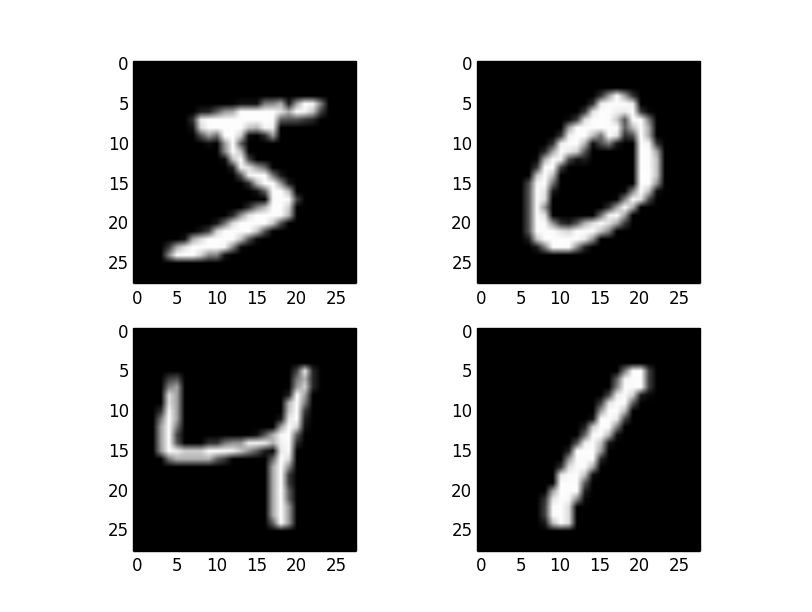
\includegraphics[width=2.60417in]{mnist_details.png}
\caption{Reconnaissance de chiffres écrits à la main}
\end{figure}

\begin{itemize}
\tightlist
\item
  Chaque image \(i\) de chiffre est de taille \(28 \times 28 = 784\)
  pixels
\item
  A chaque pixel \(j\) est associé un niveau de gris
  \(x_i^j \in \{0,\dots, 255\}\)
\end{itemize}

\end{frame}

\begin{frame}{Example 1: reconnaissance de chiffres}

\begin{itemize}
\item
  Les niveaux de gris stockés dans un vecteur
  \(\mathbf{x}_i = (x_i^r)_{r=1\dots p}\), \(p=784\)
\item
  \(y_i \in \{0,\dots, 9\}\) : étiquette de l'image

  \begin{itemize}
  \tightlist
  \item
    \(y_i\) connu pour un échantillon d'apprentissage
  \item
    \(y\) doit être prédit pour une nouvelle image \(\mathbf{x}\)
  \end{itemize}
\end{itemize}

\end{frame}

\begin{frame}{Formellement}

\begin{itemize}
\item
  On considère \(n\) objets (images, textes, son\ldots{}), décrits par
  \(p\) caractéristiques.
\item
  Pour chaque objet \(i\), ces caractéristiques sont stockées dans un
  vecteur \(\mathbf{x}_i = (x_i^1, \dots, x_i^p)\) de \(\mathbb{R}^p\).
\item
  A chaque objet \(i\) est affectée une variable de sortie \(y_i\).

  \begin{itemize}
  \tightlist
  \item
    Si \(y_i \in \mathbb{R}^p\) : on parle de régression
  \item
    Si \(y_i \in E\) avec \(E\) ensemble fini on parle

    \begin{itemize}
    \tightlist
    \item
      de discrimination si \(E = \{0,1\}\);
    \item
      de classement si \(E=\{0,\dots, 9\}\) par exemple
    \item
      de reconnaissance de forme si
      \(E=\{\text{chien},\text{marmotte},...\}\)
    \end{itemize}
  \end{itemize}
\item
  \textbf{But}: prédire la sortie \(y\) pour un nouvel ensemble de
  caractéristiques \(\mathbf{x}\)
\item
  \textbf{Comment}: apprendre (sur un jeu de données d'apprentissage =
  training) une règle de prédiction ou classification et fournir cette
  règle pour l'appliquer à \(\mathbf{x}\)
\end{itemize}

\end{frame}

\begin{frame}{Autres exemples}

\begin{itemize}
\tightlist
\item
  Reconnaissances de visages sur des photos \(E = \{\)membres d'une
  famille \(\}\)
\item
  Reconnaissance du bord politique par l'analyse des discours
\end{itemize}

\end{frame}

\begin{frame}{Différence entre estimation ou apprentissage?}

\begin{itemize}
\tightlist
\item
  Tradition statistique / estimation :

  \begin{itemize}
  \tightlist
  \item
    Notion de modèle centrale avec une finalité explicative
  \item
    Cherche à approcher la réalité, modèle éventuellement basé sur une
    théorie physique, économique,
  \item
    Interprétation du rôle de chaque variable explicative prépondérante
    dans la démarche.
  \end{itemize}
\item
  Apprentissage : l'objectif est essentiellement la prédiction,

  \begin{itemize}
  \tightlist
  \item
    meilleur modèle n'est pas nécessairement celui qui ajusterait le
    mieux le vrai modèle.
  \item
    cadre théorique est différent et les majorations d'erreur requièrent
    une autre approche : choix basés sur des critères de qualité de
    prédiction
  \item
    l'interprétabilité passe au deuxième plan.
  \end{itemize}
\end{itemize}

\end{frame}

\begin{frame}{Et le bon vieux modèle linéaire (généralisé) dans tout
ça?}

\[ y_i \sim  \mathcal{F} \quad \mbox{ avec } \quad \phi(\mathbb{E}[y_i]) = \mathbf{x}^T\beta\]

\begin{itemize}
\tightlist
\item
  Si les dimensions du problèmes \((n, p)\) sont raisonnables
\item
  Si les hypothèses relatives au modèle (linéarité) et aux distributions
  sont vérifiées
\item
  ALORS : les techniques statistiques de modélisation tirées du modèle
  linéaire général sont optimales (maximum de vraisemblance)
\item
  On ne fera pas mieux, surtout dans le cas d'échantillons de taille
  restreinte
\end{itemize}

\end{frame}

\begin{frame}{MAIS}

\begin{itemize}
\tightlist
\item
  Dès que les hypothèses distributionnelles ne sont pas vérifiées,
\item
  Dès que les relations supposées entre les variables ou la variable à
  modéliser ne sont pas linéaires
\item
  Dès que le volume des données (big data) est important,
\end{itemize}

On se tournera vers d'autres méthodes qui viennent concurrencer les
modèles statistiques rudimentaires.

\end{frame}

\section{Deep learning}\label{deep-learning}

\begin{frame}{Deep learning: introduction}

\begin{itemize}
\tightlist
\item
  Définition (tentative): ensemble de méthodes d'apprentissage cherchant
  à modéliser les données avec des architectures complexes combinant
  diverses transformations non-linéaires.
\end{itemize}

\[ \mathbf{x} \mapsto f(\mathbf{x},\theta) \mbox{ telle que } 
y \simeq f(\mathbf{x},\theta)\]

\begin{itemize}
\tightlist
\item
  Les briques élémentaires du Deep Learning sont les \textbf{réseaux
  neuronaux}.
\item
  Ces briques sont combinées pour former des \textbf{réseaux de neurones
  profonds}.
\end{itemize}

\end{frame}

\begin{frame}{Domaines d'application}

Ces techniques ont permis des progrès significatifs dans les domaines
suivants:

\begin{itemize}
\tightlist
\item
  traitement d'image et de son : reconnaissance faciale, reconnaissance
  automatique de la parole (transformation d'une voix en texte écrit),
\item
  vision par ordinateur : imiter la vision humaine (machine voyant
  plusieurs objets à la fois)
\item
  Traitement automatique du langage naturel
\item
  Classification de textes (par exemple détection de spam)
\end{itemize}

Quantité infinie d'applications potentielles

\end{frame}

\begin{frame}{Différentes types d'architectures pour les réseaux
neuronaux}

\begin{itemize}
\item
  \emph{Les perceptrons multicouches} : les plus vieux et les plus
  simples
\item
  \emph{Les réseaux neuronaux convolutifs} : très performants pour le
  traitement d'image
\item
  \emph{Les réseaux neuronaux récurrents}, utiles pour les données
  séquentielles (textes ou séries temporelles)
\item
  Tous sont basés sur des cascades profondes de couches
\item
  Requiert des algorithmes d'optimisation intelligents (stochastiques en
  général), une initialisation minutieuse et un choix malin de
  structure.
\item
  Résultats impressionnnants mais peu de justifications théoriques pour
  l'instant
\end{itemize}

\end{frame}

\begin{frame}{Neurone artificiel}

\begin{itemize}
\item
  \textbf{Un neurone} est une application non linéaire en ses paramètres
  qui, à un vecteur \(\mathbf{x}\) d'entrée associe une sortie
  \(f(\mathbf{x})\) :
\item
  Plus précisément, le \(j\)-ième neurone artificiel \(f_j\) s'écrit
  \[f_j(\mathbf{x}) = \phi(<w_j,\mathbf{x}> + b_j)\]
\end{itemize}

où

\begin{itemize}
\item
  \(<w_j,\mathbf{x}> = \sum_{r=1}^p w_j^r x^r\)
\item
  Les quantités \(w_j = (w_j^1,\dots,w_j^p)\) pondèrent les variables
  d'entrée \((x^1, \dots,x^p)\)
\item
  \(b_j\) est appelé le biais du neurone \(j\).
\item
  \(\phi\) est appelée fonction d'activation
\end{itemize}

\end{frame}

\begin{frame}{Modèle basique à un neurone}

On explique la variable de sortie \(y\) par
\[ y \simeq f(\mathbf{x},\theta) =  \phi(<w,\mathbf{x}> + b)\]

Si \(\phi(z) =z\) et un seul neurone \(\Rightarrow\) modèle linéaire
simple

\end{frame}

\begin{frame}{Choix de la fonction d'activation \(\phi\)}

\begin{itemize}
\item
  Si \(Y \in \{0,1\}\) et on souhaite prédire \(P(Y=1|x)\) : la
  logistique \(\phi(z) = \frac{1}{1+e^{-z}} \in [0,1]\)
\item
  \emph{Généralisation}: Si \(Y \in E\) (\(E\) espace fini) et
  prédiction de \(P(Y= e|x)\) : \(softmax\)
  \[\phi(z) =\left(\frac{e^{z_e}}{\sum_{e \in E} e^{z_e}}\right)_{e \in E}\]
\item
  La fonction tangente hyperbolique:
  \(\phi = \tanh:\mathbb{R} \mapsto [-1,1]\)
\item
  La fonction de seuil: \(\phi(z) = 1_{z>s} \in \{0,1\}\)
\item
  La partie positive: \textbf{rectified linear unit (ReLU)}
  \(\phi(z) = max(z,0)\)

  \begin{itemize}
  \tightlist
  \item
    Permet de prédire des valeurs positives. Continue mais non dérivable
  \end{itemize}
\end{itemize}

\end{frame}

\begin{frame}{Propriétés}

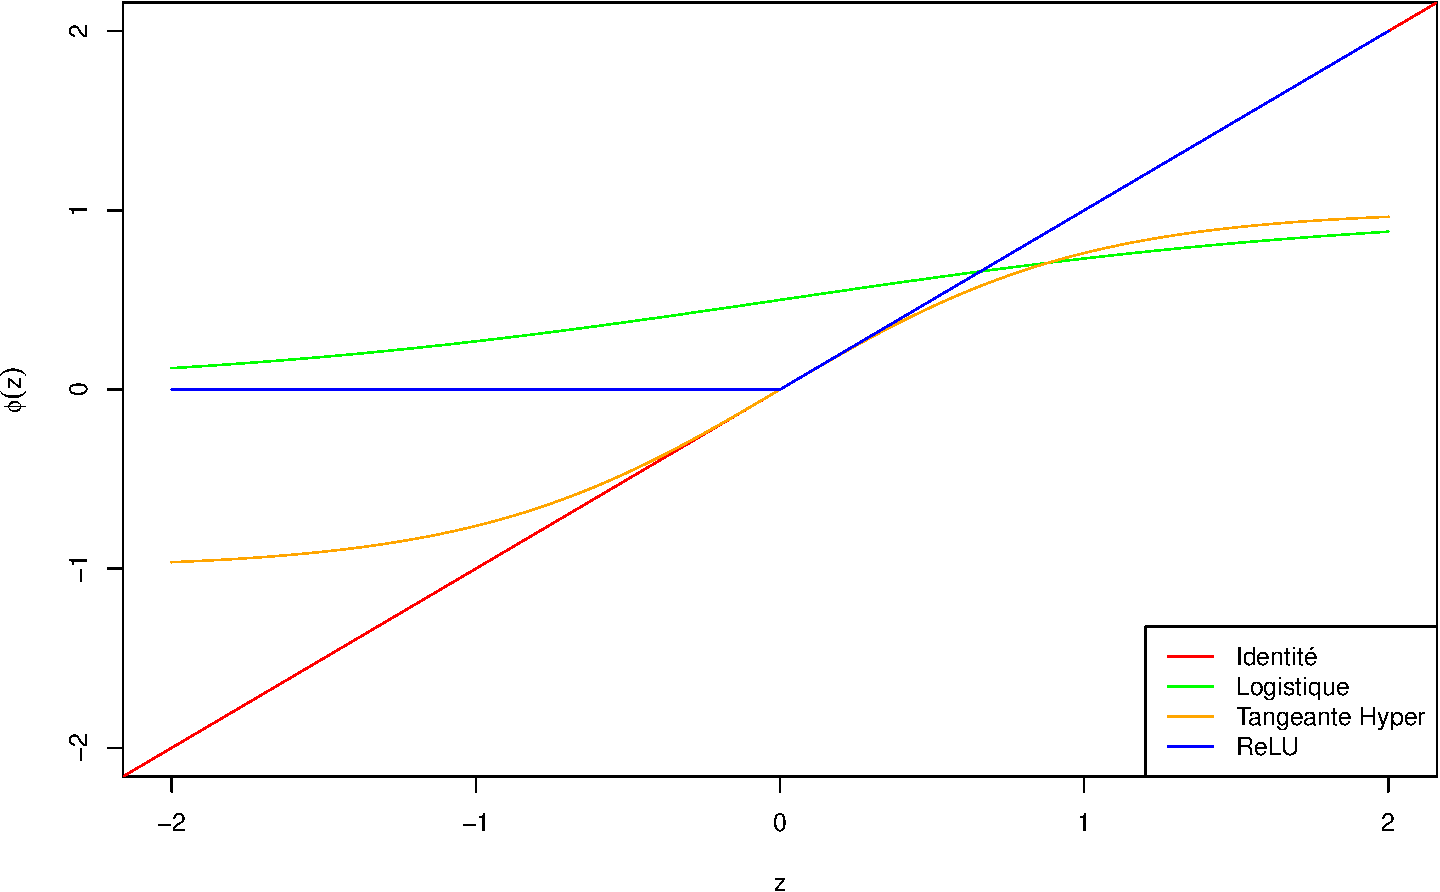
\includegraphics{cours_deeplearning_for_dummies_files/figure-beamer/unnamed-chunk-1-1.pdf}

Différentes propriétés de différentiabilité : important au moment de
l'optimisation des \(w\) et \(b\)

\end{frame}

\begin{frame}{Réseaux de neurones ou perceptrons multicouches}

\begin{itemize}
\tightlist
\item
  Structure composée de différentes couches cachées de neurones dont la
  sortie sert d'entrée aux neurones de la couche suivante
\item
  Les fonctions d'activations sont les mêmes dans les différentes
  couches, seule la dernière est différente (à adapter à l'objectif :
  classification ou régression)
\end{itemize}

\end{frame}

\begin{frame}{Exemple}

\begin{figure}
\centering
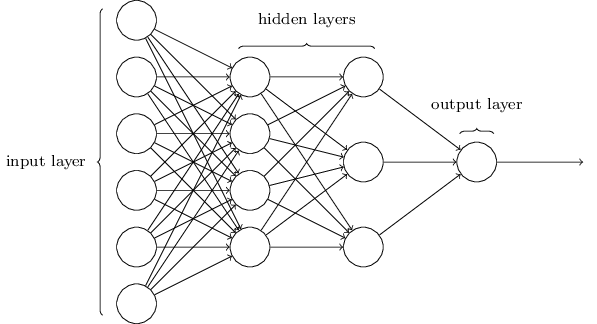
\includegraphics[width=2.60417in]{mlp-network.png}
\caption{Example de réseau de neurones}
\end{figure}

\begin{itemize}
\tightlist
\item
  Input layer : autant de noeuds que de variables \(x^r\) : \(p\)
\item
  Hidden layer : nombre de neurones à fixer (ici 4 puis 3)
\item
  Output layer : 1 noeud = \(y\)
\end{itemize}

\end{frame}

\begin{frame}{Réseau de neurones: formellement}

On note \(J_{\ell}\) le nombre de neurones de la couche \(\ell\)

\begin{itemize}
\item
  Couche \(0\) : \(h^0(\mathbf{x}) = \mathbf{x} \in \mathbb{R}^p\)
\item
  Pour les couches cachées \(\ell = 1\dots L\):

  \begin{itemize}
  \item
    On crée \(J_{\ell}\) neurones : pour tout \(j = 1 \dots J_{\ell}\) :

    \begin{eqnarray*}
    a^{(\ell)}_j(\mathbf{x}) &=& b^{(\ell)}_j + \sum_{m=1}^{J_{\ell-1}} W^{(\ell)}_{jm} h_m^{(\ell-1)}(\mathbf{x}) \\
    &=& b^{(\ell)}_j + < W^{(\ell)}_{j},  h ^{(\ell-1)}(\mathbf{x}) >
    \end{eqnarray*}

    \[h_j^{(\ell)}(\mathbf{x}) = \phi(a_j^{(\ell)}(\mathbf{x}))\]
  \item
    Vectoriellement :
    \[a^{(\ell)}(\mathbf{x}) = b^{(\ell)} +W^{(\ell)} h^{(\ell-1)}(\mathbf{x}) \in \mathbb{R}^{J_{\ell}}\]
    \[h^{(\ell)}(\mathbf{x}) = \phi(a^{(\ell)}(\mathbf{x}))\] où
    \(W^{(\ell)}\) est une matrice \(J_{\ell} \times J_{\ell-1}\)
  \end{itemize}
\end{itemize}

\end{frame}

\begin{frame}{Réseau de neurones: formellement}

\begin{itemize}
\item
  Pour la dernière couche : \(\ell = L+1\):

  \[a^{(L+1)}(\mathbf{x}) = b^{(L+1)} +W^{(L+1)} h^{(L)}(\mathbf{x}) \in \mathbb{R}^J\]

  \[h^{(L+1)}(\mathbf{x}) = \psi(a^{(L+1)}(\mathbf{x}))\]
\end{itemize}

\end{frame}

\begin{frame}{Réseau de neurones: finalement}

\begin{itemize}
\tightlist
\item
  \(W^{(\ell)}\) est une matrice de poids de taille \(J_{\ell}\) lignes
  et \(J_{\ell-1}\) colonnes
\item
  \(W^{(L+1)}\) est une matrice de poids de taille \(1\) lignes et
  \(J_{L}\) colonnes si \(y \in \mathbb{R}\)
\item
  \[\mathbf{x} \mapsto f(\mathbf{x},\theta) = \psi(a^{(L+1)}(\mathbf{x}))\]

  \begin{itemize}
  \tightlist
  \item
    Si on fait de la régression \(\psi(z) = z\),
  \item
    Si on fait de la classification en deux classes, \(\psi\) est la
    sigmoïde (prédiction dans \([0,1]\)).
  \item
    Si on fait de la classification en plusieurs classes :
    \(\psi = softmax\)
  \end{itemize}
\end{itemize}

\end{frame}

\begin{frame}{Réseau de neurones:}

\begin{itemize}
\item
  Architecture basique puisque chaque couche dépend de la couche
  précédente et non des neurones de la même couche (\(\Rightarrow\)
  réseaux de neurones récurrents)
\item
  Paramètres de l'architecture:

  \begin{itemize}
  \tightlist
  \item
    nombre de couches
  \item
    nombre de neurones dans chaque couche
  \item
    fonctions d'activation des couches cachées (\(\phi\)) et de la
    dernière (\(\psi\))
  \end{itemize}
\item
  Pour la dernière fonction \(\psi\), guidé par le problème

  \begin{itemize}
  \tightlist
  \item
    Si régression : \(\psi = id\) ou \(g\)
  \item
    Si classification sigmoide (\(\{0,1\}\)) ou softmax (classification
    avec plus de deux catégories)
  \end{itemize}
\end{itemize}

\end{frame}

\begin{frame}{Réseaux neuronaux récurrents}

\begin{itemize}
\tightlist
\item
  La sortie d'un neurone peut service d'entrée à un neurone de la même
  couche ou d'une couche précédente.
\end{itemize}

\end{frame}

\begin{frame}{Justification théorique}

Hornik (1991) a prouvé que toute fonction régulière bornée de
\(\mathbb{R}^p\) dans \(\mathbb{R}\) peut être approchée pour un réseau
de neurones avec une couche cachée contenant un nombre fini de neurones
et ayant la même fonction d'activation et \(\psi = id\).

\begin{itemize}
\item
  Théorème intéressant d'un point de vue théorique
\item
  En pratique : nombre de neurones de la couche cachée peut être très
  grand.
\item
  Force du deep learning : dans le nombre de couches cachées
\end{itemize}

\end{frame}

\section{Estimation des paramètres}\label{estimation-des-parametres}

\begin{frame}{Quantité à minimiser}

Etant donnée une fonction de perte \(\ell(f(\mathbf{x},\theta),Y\),

Risque (erreur de prédiction) :
\[\mathbb{E}_{Y}[\ell(f(\mathbf{x},\theta),Y)]\]

\end{frame}

\begin{frame}{Fonction de perte}

\begin{itemize}
\tightlist
\item
  Paramètres à estimer : \(\theta\) = poids \(W^{(\ell)}\) et biais
  \(b^{(\ell)}_j\)
\item
  Classiquement : estimation par maximisation de la
  (\(\log\))-vraisemblance
\item
  Fonction de perte: \(=-\log\;\)vraisemblance

  \begin{itemize}
  \item
    Cas de la régression :
    \(Y \sim \mathcal{N}(f(\mathbf{x},\theta), I)\)
    \[ \ell(f(\mathbf{x},\theta),Y) = \| Y - f(\mathbf{x},\theta)\|^2\]
  \item
    Cas de la classification \(\{0,1\}\) :
    \(Y \sim \mathcal{B}(1,f(\mathbf{x},\theta))\)
    \[ \ell(f(\mathbf{x},\theta),Y) = -Y \log(f(\mathbf{x},\theta)) - (1-Y) \log(1- f(\mathbf{x},\theta))\]
    (cross-entropy)
  \item
    Cas de la classification multiclasses
    \[ \ell(f(\mathbf{x},\theta),Y) =-  \sum_{e \in E} \mathbf{1}_{Y=e} \log p_{\theta}(Y = e | \mathbf{x} )\]
  \end{itemize}
\end{itemize}

\end{frame}

\begin{frame}{Fonction de perte : remarque}

\begin{itemize}
\item
  Idéalement on voudrait minimiser l'erreur de classification mais cette
  fonction n'est pas dérivable\ldots{}
\item
  On lui préfèrera la ``cross-entropy''
\end{itemize}

\end{frame}

\begin{frame}{Risque empirique pénalisé}

\begin{itemize}
\item
  \(\mathbb{E}_{Y}[\ell(f(\mathbf{x},\theta),Y)]\) remplacé par risque
  empirique
\item
  Pour un échantillon d'entraînement \((\mathbf{x}_i,Y_i)_{i=1\dots n}\)
\end{itemize}

\[ L_n(\theta) = \frac{1}{n}\sum_{i=1}^n  \ell(f(\mathbf{x}_i,\theta),Y_i)\]

\begin{itemize}
\tightlist
\item
  Pénalisation :
  \[ L_n(\theta) = \frac{1}{n}\sum_{i=1}^n  \ell(f(\mathbf{x}_i,\theta),Y_i) + \lambda \Omega(\theta) \]
  avec par exemple
  \(\Omega(\theta) = \sum_{\ell,i,j} (W^{(\ell)}_{ij})^2\) ou
  \(\Omega(\theta) = \sum_{\ell,i,j} |W^{(\ell)}_{ij}|\)
\end{itemize}

\end{frame}

\begin{frame}{Minimisation par descente de gradient stochastique.
Rumelhart et al (1988)}

\begin{itemize}
\item
  Choisir un vecteur initial de paramètres \(\theta\), et un taux
  d'apprentissage \(\eta\)
\item
  Répéter jusqu'à ce qu'un minimum approché (assez précisément) soit
  obtenu:

  \begin{itemize}
  \tightlist
  \item
    Diviser aléatoirement l'échantillon d'apprentissage en \(N_B\)
    sous-échantillons (batch) de taille \(m\) (\(n = m \times N_B\))
  \item
    Pour chacun des batch \(B\) poser:
    \[ \theta:= \theta - \eta \frac{1}{m}\sum_{i \in B} \nabla_{\theta} \left\{  \ell(f(\mathbf{x}_i,\theta),Y_i) + \lambda   \Omega(\theta)\right\}\]
  \end{itemize}
\end{itemize}

\textbf{Remarques}:

\begin{itemize}
\item
  Chaque itération est appelée \emph{epoch}.
\item
  Le nombre d'epochs est un paramètre à régler.
\end{itemize}

\end{frame}

\begin{frame}{Calcul du gradient pour la régression}

\begin{itemize}
\tightlist
\item
  \(Y \in \mathbb{R}\).
\item
  \(R_i = \ell(f(\mathbf{x}_i,\theta),Y_i) = (Y_{i} - f(\mathbf{x}_i,\theta))^2\)
\item
  Fonctions d'activation \(\psi\) et \(\phi\) quelconques
\end{itemize}

\end{frame}

\begin{frame}{Dérivées partielles de \(R_i\) par rapport aux poids de la
dernière couche}

\begin{itemize}
\tightlist
\item
  Dérivées de
  \(R_i = \left(Y_{i} - f(\mathbf{x}_i,\theta)\right)^2= \left(Y_i - h^{(L+1)}(\mathbf{x}_i)\right)^2\)
  par rapport à \((W_j^{(L+1)})_{j=1\dots J_{L}}\)
\end{itemize}

\begin{itemize}
\item
  \begin{eqnarray*}
  f(\mathbf{x} ,\theta) &=& h^{(L+1)}(\mathbf{x}) \\
  &=& \psi(a^{(L+1)}(\mathbf{x}))  \\
  & =& \psi\left(b^{(L+1)} +\sum_{j=1}^{J_L} W_j^{(L+1)} h_j^{(L)}(\mathbf{x}) \right)
  \end{eqnarray*}
\item
  \[ \frac{\partial R_i }{\partial W^{(L+1)}_{j}} = -2\left(Y_{i} - f(\mathbf{x}_i,\theta)\right)\psi'\left(a^{(L+1)}(\mathbf{x}_i)\right)h_j^{(L)}(\mathbf{x}_i)\]
\end{itemize}

\end{frame}

\begin{frame}{Dérivées partielles de \(R_i\) par rapport aux poids de
l'avant-dernière couche}

\begin{itemize}
\item
  Dérivées de \(R_i = \left(Y_i - h^{(L+1)}(\mathbf{x}_i)\right)^2\) par
  rapport à \((W_{jm}^{(L)})_{j=1\dots J_{L},m=1\dots J_{L-1}}\)
\item
  \begin{eqnarray*}
  \frac{\partial R_i }{\partial W^{(L)}_{jm}} &=& -2\left(Y_{i} - f(\mathbf{x}_i,\theta)\right)\psi'\left(a^{(L+1)}(\mathbf{x}_i)\right) \frac{\partial}{\partial W^{(L)}_{jm}}  a^{(L+1)}(\mathbf{x}_i)
  \end{eqnarray*}
\end{itemize}

\end{frame}

\begin{frame}{Dérivées partielles de \(R_i\) par rapport aux poids de
l'avant-dernière couche}

\begin{eqnarray*} 
a^{(L+1)}(\mathbf{x}) &=&  b^{(L+1)} + \sum_{j=1}^{J_L} W^{(L+1)}_j h_j^{(L)}(\mathbf{x}) \\
&=&  b^{(L+1)} + \sum_{j=1}^{J_L}  W^{(L+1)}_j \phi \left(b_j^{(L)} + \sum_{m=1}^{J_{L-1}} W^{(L)}_{jm} h_m^{(L-1)}(\mathbf{x})\right)
\end{eqnarray*}

\begin{eqnarray*}
\frac{\partial}{\partial W^{(L)}_{jm}}  a^{(L+1)}(\mathbf{x}_i)  &=&   W^{(L+1)}_j \phi' \left(b_j^{(L)} + \sum_{m=1}^{J_{L-1}} W^{(L)}_{jm} h_m^{(L-1)}(\mathbf{x}_i)\right) \\
&& \times h_m^{(L-1)}(\mathbf{x}_i)   \\
&=& W^{(L+1)}_j \phi'(a_j^{L}(\mathbf{x}_i)) h_m^{(L-1)}(\mathbf{x}_i)
\end{eqnarray*}

\end{frame}

\begin{frame}{Forward Backward (en travaillant un peu) (à chaque
itération)}

\begin{itemize}
\tightlist
\item
  Etant données des paramètres courant
\item
  \textbf{Etape de forward} : De la couche \(1\) vers la couche \(L+1\),
  on calcule les
  \(a_j^{\ell}(\mathbf{x}_i),\phi(a_j^{\ell}(\mathbf{x}_i))\)
\item
  \textbf{Etape de backward} : De la couche \(L+1\) vers la couche
  \(1\), on calcule les dérivées partielles (formule de mise à jour par
  récurrence)
\end{itemize}

\end{frame}

\begin{frame}{Réglages de l'algorithme}

\begin{itemize}
\item
  \(\eta\): taux d'apprentissage de la descente de gradient

  \begin{itemize}
  \tightlist
  \item
    si \(\eta\) trop petit, convergence très lente avec possiblement
    atteinte d'un minimum local
  \item
    si \(\eta\) trop grand, oscillation atour d'un optimum sans
    stabilisation
  \item
    choix adaptatif du \(\eta\) (\(\eta\) décroissant)
  \end{itemize}
\item
  Calculs en batch permet de ne pas avoir à stocker trop de quantités
  dans le forward / backward
\item
  Evidemment multiples autres versions de l'algorithme de maximisation
  (momentum correction, Nesterov accelerated gradient, etc\ldots{})
\end{itemize}

\end{frame}

\section{Réseaux neuronaux plus
complexes}\label{reseaux-neuronaux-plus-complexes}

\begin{frame}{Réseaux neuronaux convolutifs (LeNet by LeCun et al.,
1998)}

\begin{itemize}
\item
  Lors du passage de l'image au vecteur : perte de la cohérence spatiale
  des images (formes\ldots{})
\item
  Réseaux neuronaux convolutifs ont révolutionné l'analyse d'images
  (LeCun)
\item
  CNN (convolutive neuronal networks) : composés de différentes couches
  de convolution, pooling et couches complètements connectées.
\end{itemize}

\end{frame}

\begin{frame}{En une image}

\begin{figure}
\centering
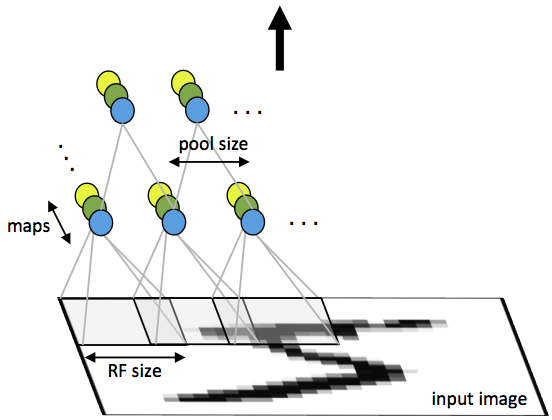
\includegraphics[width=2.60417in]{Cnn_layer_standford.png}
\caption{Architecture d'un réseau de neurone convolutif (crédit
Stanford)}
\end{figure}

\end{frame}

\begin{frame}{Couche de convolution}

\begin{itemize}
\item
  Image \(\mathcal{I}(u,v)\) : chaque pixel \((u,v)\) est décrit par
  \(C\) niveaux de couleurs (channels), par exemple RGB (bleu, vert,
  rouge) \(\Rightarrow\) tableau de taille (\(M,N,C\))
\item
  Chaque neurone basée sur une combinaison linéaire des signaux sur une
  petite région de l'image
  \[K_{u,v}*\mathcal{I}(c) =  \sum_{n=-k}^{k}\sum_{m=-k}^k K_l(n,m,c)\mathcal{I}\left(u+m,v+n,c \right)\]

  \[h_{u,v} = \phi(K_{u,v}*\mathcal{I}(c)+b_{u,v})\]
\item
  On obtient un nouveau neurone en déplaçant cette fenêtre

  \begin{itemize}
  \tightlist
  \item
    si on déplace peu : redondance de l'information
  \item
    si on déplace beaucoup : perte d'information
  \end{itemize}
\end{itemize}

\end{frame}

\begin{frame}{Couche de pooling (subsampling)}

\begin{itemize}
\tightlist
\item
  Faire des moyennes ou prendre des max sur des petites régions
\item
  \(\phi\) peut être appliquée avant ou après le pooling
\item
  Permet de réduire la dimension (nombre de variables à traîter) mais
  aussi de rendre le réseau moins sensible aux translations éventuelles
  de l'image
\end{itemize}

\end{frame}

\begin{frame}{Ensuite}

\begin{itemize}
\tightlist
\item
  Après plusieurs couches et convolution / pooling, on applique une ou
  plusieurs couches des \emph{fully connected layers} (= réseau montré
  avant)
\end{itemize}

\end{frame}

\begin{frame}{Vers des architectures de réseaux de plus en plus
complexes}

\begin{itemize}
\item
  Réseaux maintenant beaucoup plus complexes
\item
  Possible de le traiter grâce aux cartes GPU (Graphical Processor Unit)
\item
  Résultats du \emph{Large Scale Visual Recognition Challenge (ILSVRC)}
\end{itemize}

\begin{figure}
\centering
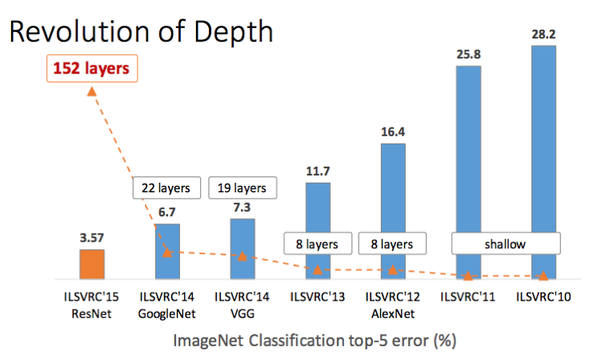
\includegraphics[width=2.60417in]{depth_error.png}
\caption{Taux d'erreur et nombre de couches}
\end{figure}

\end{frame}

\section{Conclusion}\label{conclusion}

\begin{frame}{Conclusion}

\begin{itemize}
\tightlist
\item
  Vision ultra-rapide de la définition d'un réseau de neurones profonds
\item
  En pratique : expertise repose sur comment combiner les couches et les
  différents types de neurones
\item
  Références :

  \begin{itemize}
  \tightlist
  \item
    Wikipédia
  \item
    Cours de Wikistat par Philippe Besse (Toulouse)
  \item
    Livre de référence : Deep Learning de Yoshua Bengio
  \end{itemize}

  \begin{figure}
  \centering
  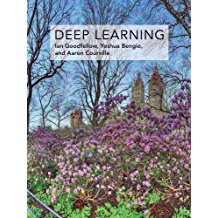
\includegraphics[width=0.52083in]{livre_bengio.jpg}
  \caption{Ouvrage de référence}
  \end{figure}

  \begin{itemize}
  \tightlist
  \item
    Vidéo
    \url{https://www.college-de-france.fr/site/yann-lecun/course-2016-02-12-14h30.htm}
  \item
    Résultats et exposés de Francis Bach
  \end{itemize}
\end{itemize}

\end{frame}

\end{document}
